\documentclass[letterpaper]{article}
\usepackage{a4wide}
\usepackage{arxiv}
\usepackage[OT1]{fontenc} 
\usepackage{hyperref}
\usepackage{bookmark}       % hyperlinks
\usepackage{url}            % simple URL typesetting
\usepackage{booktabs}       % professional-quality tables
\usepackage{amsmath,amsfonts}       % blackboard math symbols
\usepackage{cleveref}
\usepackage{nicefrac}       % compact symbols for 1/2, etc.
\usepackage{microtype}      % microtypography
\usepackage{lipsum}
\usepackage{graphicx}
\newcommand{\F}{\mathcal{F}}
\newcommand{\X}{\mathcal{X}}
\newcommand{\xvec}{\mathrm{x}}
\usepackage[backend=biber]{biblatex}
\addbibresource{references.bib}
\title{ALASKA2: Image Steganalysis Competition. A Final Project Report}

\author{
    Ilia Ilmer \\
  Graduate Center CUNY \\
  Department of Computer Science \\
  \texttt{iilmer@gradcenter.cuny.edu} \\
}

\begin{document}
\maketitle
\begin{abstract}
    In May of 2020, Troy University of Technology organized a competition on Kaggle.com titled ``ALASKA2: Detect secret data hidden within digital images''. The goal of the competition is to predict presence of hidden data in a particular image.
    In this project, we will identify reliable and promising convolutional neural network based models that will help me in solving the task. I will define the task as a multi-class classification problem to simplify the approach. In the process of solving the problem we will apply various deep learning training techniques in order to maximize the score. As a result of methods applied here, the score allowed us to score in top 20\% of all participants and as of May 17th, 2020, this was considered a bronze tier.
\end{abstract}

\section{Introduction}

Steganalysis is a scientific discipline that studies various forms of data in order to determine whether or not a secret message is concealed in that data. It allows communication through means that are indistinguishable from regular exchanges of information. Researchers working on discovering hidden information through steganalysis use setups that do not necessarily resemble real-life occurrences. The aspects of message encoding such as methods and parameters used are often known in advance, the data is clean, taken from a single resource using the same camera settings for all images.

In real life, message decoding is a much harder task to solve. This competition aims to simulate a realistic scenario in which 3 types of encoding are used. A dataset 75,000 unique 512 by 512 color images have been used as a cover for secret messages. The data were obtained from different sources with different quality settings.

There are three unique ways the message is encoded into the image for us, JMiPOD~\cite{jmipod}, JUNIWARD~\cite{juniward}, and UERD~\cite{uerd}. Each method is applied to all 75,000 original covers creating in total 225,000 images that have encodings of different types. Encoding is done using the JPEG compression algorithm. More specifically, during the JPEG compression, the message is encoded through DCT coefficients and is hidden from the viewer.

The JUNIWARD algorithm is exploiting the linearity of discrete cosine transform and linear transformation of Gaussian random variables. In order to minimize detectability, the algorithm solves an optimization problem with respect to pixel values obtained from inverse DCT.\@JMiPOD method utilizes the approach of bitwise encoding. The image is converted to binary codes and the message is encoded into these codes bitwise. Finally, UERD also utilizes DCT coefficients during encoding.

The following report is organized as follows. We formulate a machine learning problem presented to us as a multi-class classification task in section 2. In section 3 we perform simple data exploration and analysis. In section 4, we describe the model selection algorithm and hyperparameter tuning as well as the training setup and tricks. In that same section we also report the results of the training and the leaderboard score obtained so far. Finally, we list further ways of improvement in the final section.

\section{Task Formulation}

In this section we will pose the steganalysis detection problem as a classification. The general topic of image classification has been widely explored in the modern era of machine learning. Computational hardware allows one to implement various efficient and extremely powerful techniques, especially algorithms for dealing with thousands of images in one training session.

As such, the current competition deals with images as well. We are thus motivated to apply  and take advantage of reliable neural network architectures available as parts of PyTorch or Tensorflow packages. Computer vision has recently tremendously benefitted from deep neural network applications, gaining momentum not only in the academic world, but in the industry. Advanced architectures can to catch intricate differences between an image with one encoding or another. This is achieved by learning representations of pixels through optimization of multiple parameters of the network at ones (i.e.\ the weights).

Let us pose the competition problem as a 4-class classification task in the following manner. We are given to consider a dataset of 300,000 images of which there are 4 classes
\[ \begin{cases}
        0 -\text{cover},     \\
        1 - \text{jmipod},   \\
        2 - \text{juniward}, \\
        3 - \text{uerd}.
    \end{cases} \]
The classes arise naturally in this setting and, furthermore, they are perfectly balanced and we need not worry about imbalanced data when sampling.

\subsection{Competition Metric}
We train a neural network \( \F \) on the aforementioned collection of images \( \X = \{ \xvec_k: k=0,1,2,3 \} \) to maximize the main metric of the competition: weighted area under ROC curve. As per the competition requirements, the submission's true positive rate values between 0 and 0.4 have weight 2 while the rest carry weight 1.

In actuality, during training we will monitor the accuracy metric as well. This is done for convenience, since the problem is posed a multi-class problem and AUC is computed for a binary classification problem. During testing, however, the following method of converting from 4-class to 2-class problem is applied. Once logits are obtained from the dictionary, we apply softmax function on them and convert them to probability-like vectors. The value at position 0 will indicate the probability that a given image is a cover. We consolidate the remaining three numbers into a sum that represents the probability of seeing a ``non-cover'' image, that is, an image with a hidden message. This allows us to obtain a vector of probabilities. We then select the probability of cover for those images that have predicted label 0, and select that of non-cover otherwise. There various other methods, including using the logits themselves, as the competition allows negative score. This method, however, was outlined by many participants and the organizers as the easiest to implement. As we can see, it also fits nicely with our multi-class setting.

\section{Data Exploration}

Let us discuss the data in question. We are studying 300,000 RGB images of size 512 by 512 pixels. For 75,000 of those images no hidden message is encoded, on the other three images, the encoding corresponds to one of three types, JMiPOD~\cite{jmipod}, JUNIWARD~\cite{juniward}, or UERD~\cite{uerd}. Each encoding utilizes the JPEG compression process and encodes the information into the DCT coefficients. This allows the message to remain hidden so much so that the difference is not reflected in the spatial domain.

In the competition description~\cite{alaska2}, the organizers provide some basic information about the data. We know that all steganalysis algorithms are applied with the same probability and that the average message length is 0.4 bits per DCT coefficient.

Let us present a random collection of images to verify that visually we are unable to observe any difference between classes. On \Cref{random} we observe random images of different classes that have different IDs. Notice the differences in quality and color. Some images are simply single color (for instance bottom right), others represent a texture (for instance, bottom middle). In this labeling, 0 represents cover, and 1, 2, 3 represent JMiPOD, JUNIWARD, UERD, respectively.


\begin{figure}
    \centering
    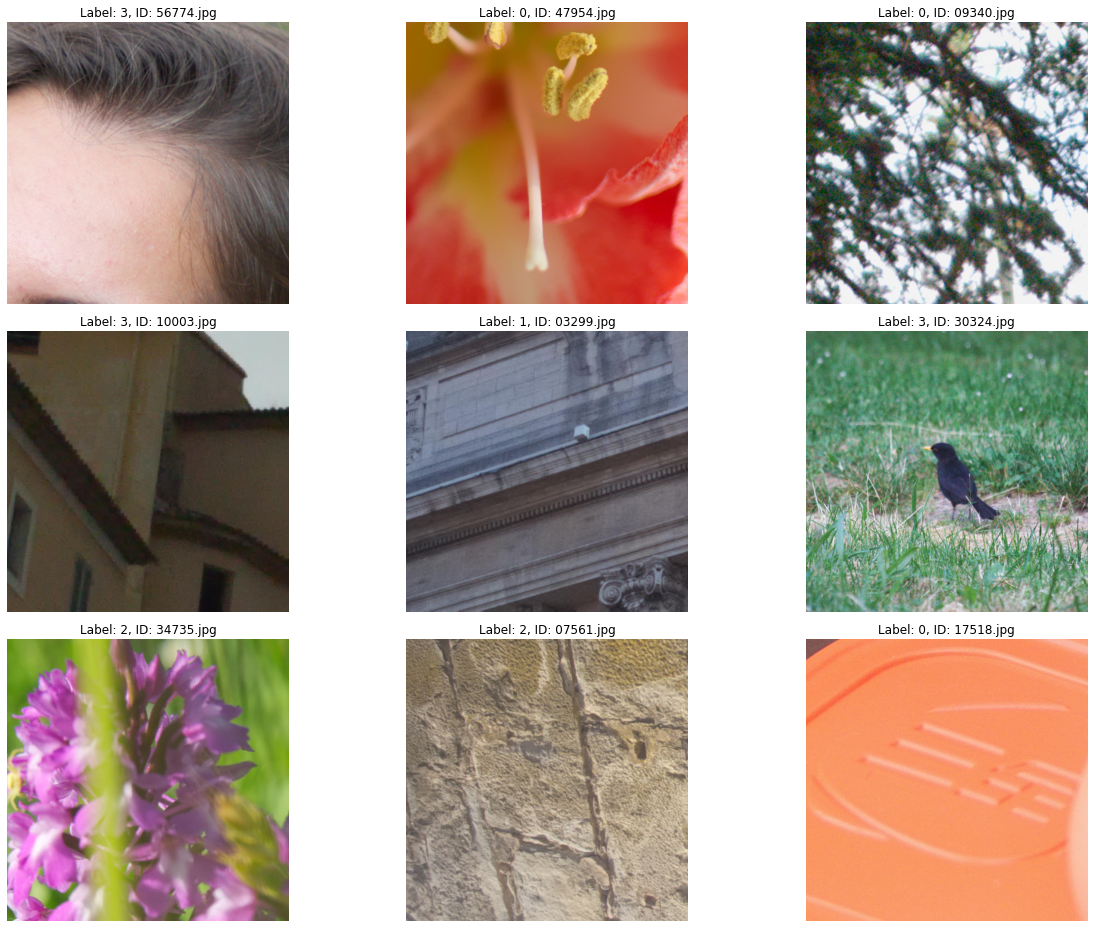
\includegraphics[width=0.75\textwidth]{random images.png}
    \caption{A random selection of images. As we ca see, no visual discrepancies between labels are observed.}
    \label{random}
\end{figure}

Next let us consider an image with a single ID, see \Cref{single}. Again, no difference is seen to us when we are dealing with RGB pixels. Let us investigate any differences in different color spaces. We are going to observe YCbCr and HSV color spaces here, for brevity.

\begin{figure}
    \centering
    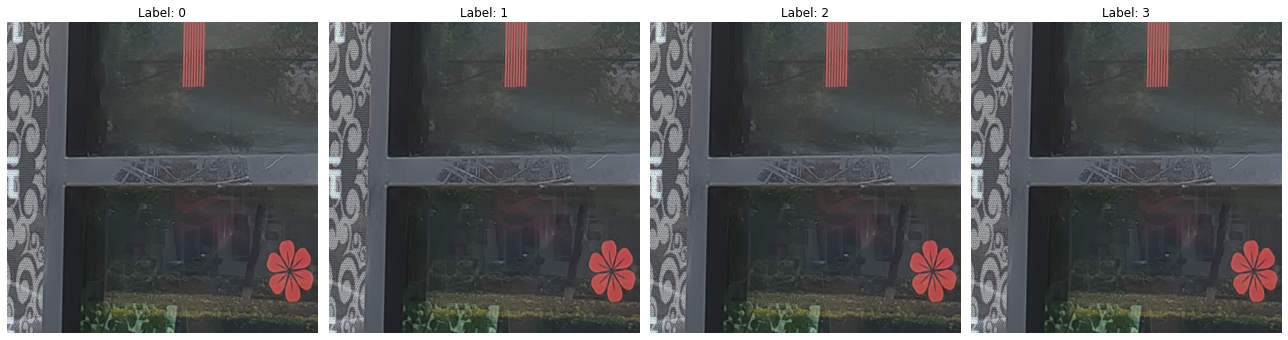
\includegraphics[width=0.75\textwidth]{four_images.png}
    \caption{A single image. Left to right: cover, JMiPOD, JUNIWARD, UERD.}
    \label{single}
\end{figure}


In YCbCr, the image is still a 3-channel array of pixel values, however, they no longer represent red, green, or blue values explicitly. Instead, the Y-channel is called luma and represents brightness of each pixel, while Cb and Cr represent difference in blue and red respectively. This transformation is obtained via linear operator. On \Cref{ycbcr} we observe each class of image represented in YCbCr color space. We seemingly do not see any difference, let us instead look at the image-wise difference between the cover and each class. This is shown on \Cref{ycbcr-difference}.

\begin{figure}
    \centering
    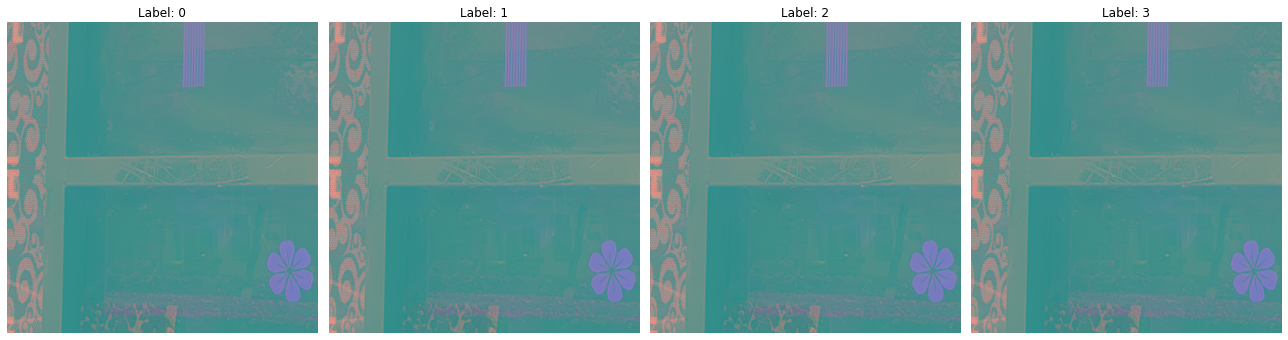
\includegraphics[width=0.75\textwidth]{same_image_ycbcr.png}
    \caption{The same image, but in YCbCr color space. Left to right: cover, JMiPOD, JUNIWARD, UERD.}
    \label{ycbcr}
\end{figure}
\begin{figure}
    \centering
    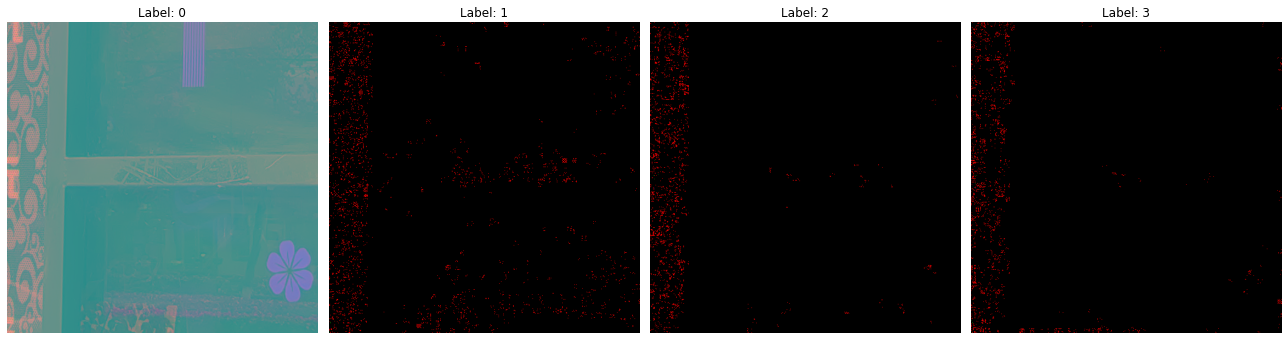
\includegraphics[width=0.75\textwidth]{difference_between_cover_noncover.png}
    \caption{The first tile shows the cover image in YCbCr color space, each subsequent tile represents the difference between the cover and a class. Left to right: cover, JMiPOD, JUNIWARD, UERD.}
    \label{ycbcr-difference}
\end{figure}

Finally, let us consider the channel-wise difference for HSV colorspace. There are channels for which the differences are more pronounced, such as Value in HSV on \Cref{ycbcr-channel-wise-hsv}, third column, last low. These values are too small in their actuality, we were unable to utilize these methods in our work.

\begin{figure}
    \centering
    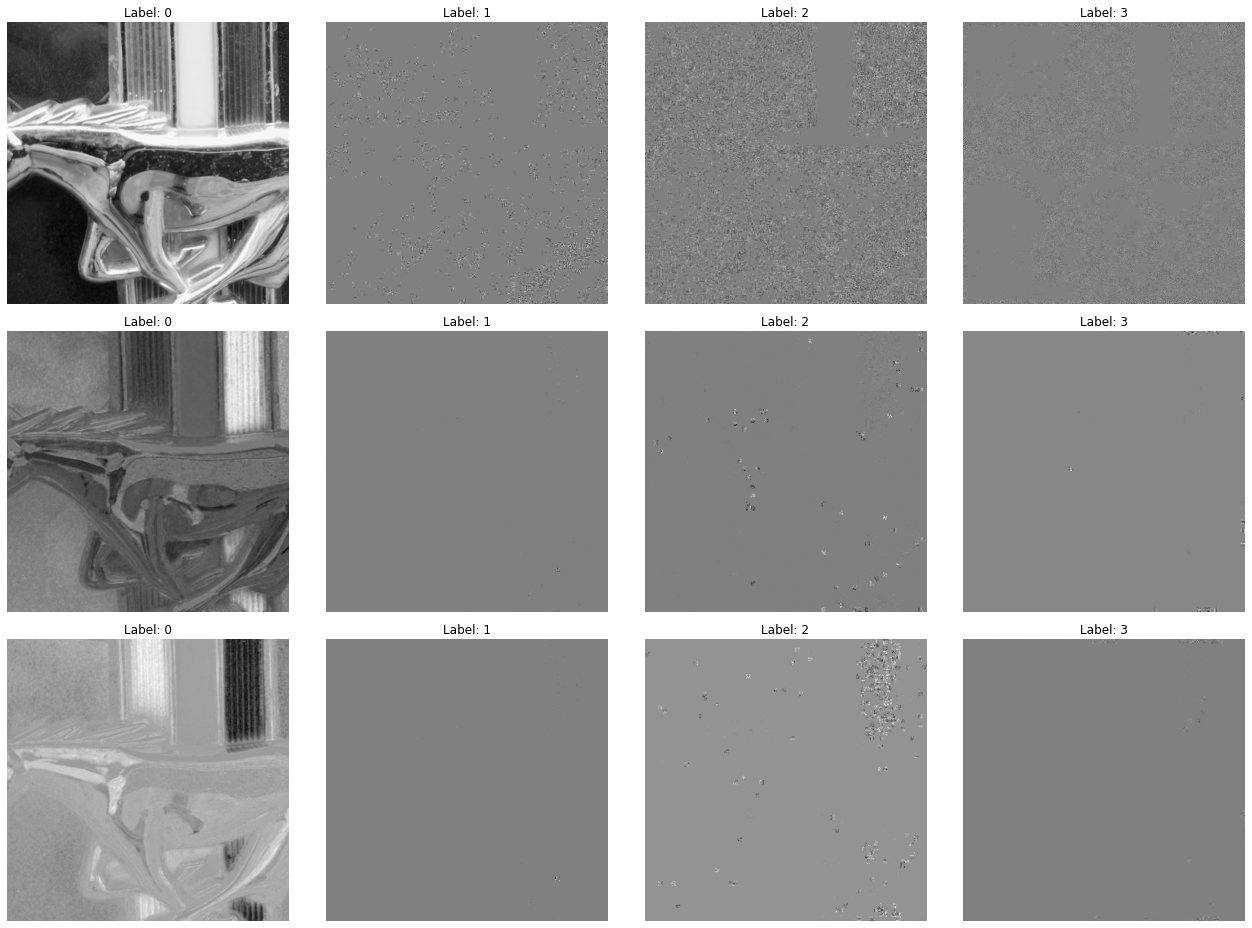
\includegraphics[width=0.75\textwidth]{channel_wise_diff.png}
    \caption{Each row represents Luma, Cr and Cb of the image. The first column is the cover HSV image. Each subsequent column is the difference between the corresponding channel of the cover and JMiPOD, JUNIWARD, or UERD.}
    \label{ycbcr-channel-wise}
\end{figure}
\begin{figure}
    \centering
    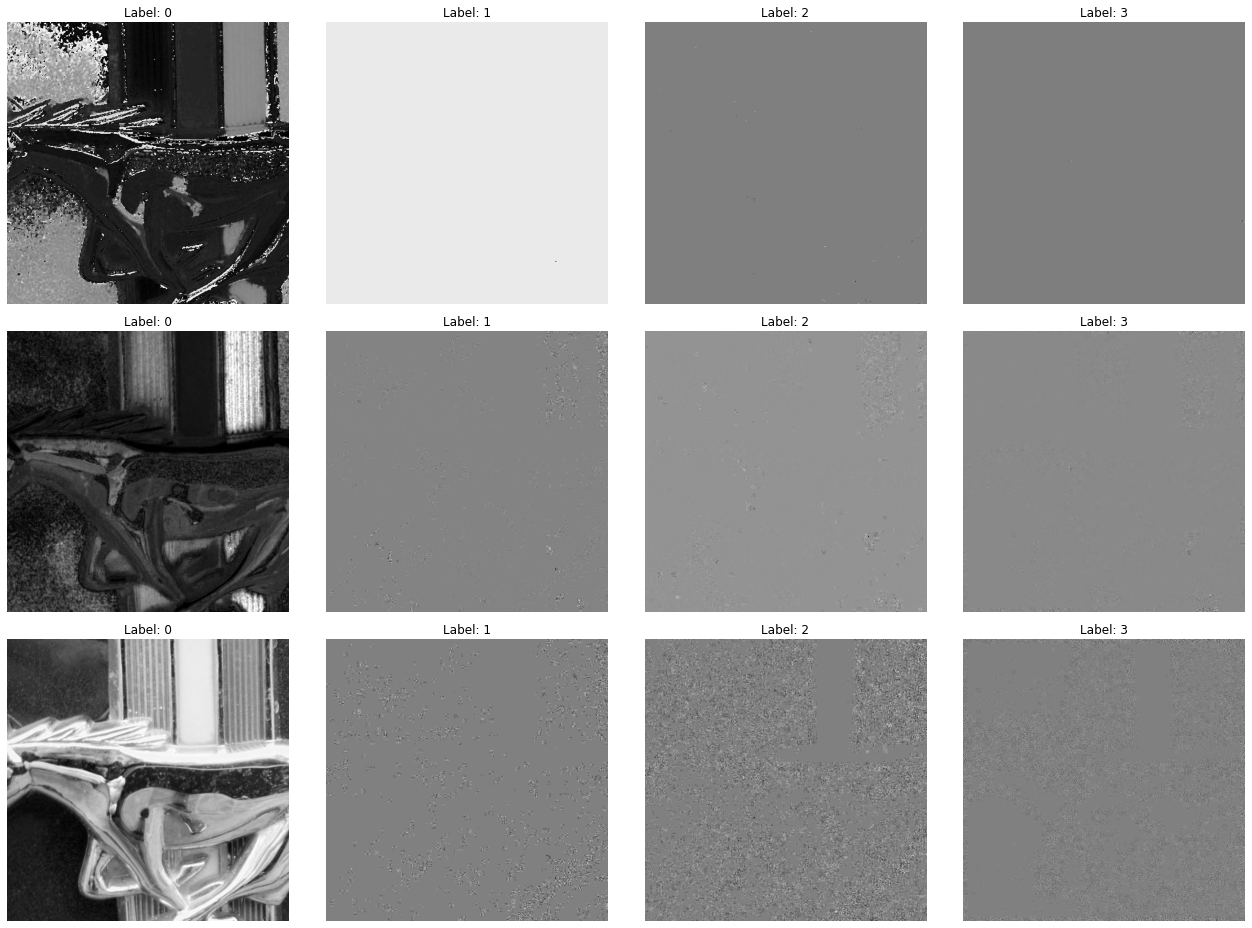
\includegraphics[width=0.75\textwidth]{channel_wise_diff_hsv.png}
    \caption{Each row represents Hue, Saturation and Value of the image. The first column is the cover HSV image. Each subsequent column is the difference between the corresponding channel of the cover and JMiPOD, JUNIWARD, or UERD..}
    \label{ycbcr-channel-wise-hsv}
\end{figure}

\section{Model Selection}

\subsection{Deep Neural Networks}

The first model we consider is the EfficientNet~\cite{tan2019efficientnet} model which is most widely used by the competitors.
This network beats state of the art results in classification and was created through an automatic architecture search algorithm. There are several versions of the network with increasing complexity and computational requirements. In this work we will experiment with a pre-trained EfficientNet-B0~\cite{tan2019efficientnet}. The network's implementation is supplied as a PyTorch based Python package available for install. The implementation provided also utilizes Swish activation function. This function was first introduced in~\cite{ramachandran2017searching} where authors considered multiple candidate-functions. Swish activation function is defined as follows

\[ Swish(x) = x\cdot \sigma(x), \]
where \( \sigma  \) is the sigmoid function. The code for this implementation is available on github as an open source package\footnote{github.com/lukemelas/EfficientNet-PyTorch/}.

The second model we will apply to the RGB images is the newly developed ResNeSt-50 model~\cite{zhang2020resnest}. The model is based on the residual structure of ResNet~\cite{he2016deep} architecture. However, the innovation is the application of the attention mechanism based on squeeze-excitation method. The input features are split into groups and within each group a further split into cardinal groups occurs. We will omit much details of the implementation described in the paper. The code for this implementation is provided by the authors\footnote{github.com/zhanghang1989/ResNeSt}. We further modify this model by replacing all rectifying linear units Swish activation function mentioned above.

The common framework for our methods is to extract features using any backbone model mentioned above and then pass these features onto a linear classifier. In this work, the classifier is a simple single-layer perceptron with softmax activation.

\subsection{Training setup}
We train the network on a machine with an NVidia RTX 2700 with 8 Gb of video memory using PyTorch with CUDA.\@ We also use a deep learning framework called Catalyst~\cite{catalyst}. Catalyst was built as a tool that abstracts away the boilerplate code of PyTorch training scheme. The overall scheme contains of four steps:
\begin{itemize}
    \item Get network outputs;
    \item Calculate loss;
    \item Calculate gradients;
    \item Update weight, set all gradients to zero.
\end{itemize}

These steps are hidden away in Catalyst. We are able to control all other aspects of training via a system of callbacks. We will state each callback we use as we go further. Let us proceed to describing the training for several models. To make the results reproducible we seed all random number generators with seed value 2020. We also set CUDA into deterministic mode using Catalyst.

\subsubsection{EfficientNet Training}

For EfficientNet-B0 configuration we use the following training approach. Firstly, we train the network on the first 16384 images from each group for 20 epochs. The training is quite time consuming, so we will train on a subset of the data, which is still a lot of data. The network is initialized as ImageNet pre-trained. We use RAdam optimizer~\cite{liu2019variance} with Lookahead wrapper~\cite{zhang2019lookahead}. RAdam is a new state-of-the-art optimizer that improves running statistics computation in Adam. Lookahead optimization algorithm is a potential improvement on the overall optimization approach. Lookahead trains the underlying optimizer, RAdam in our case, while maintaining a collection of ``faster'' weights that look ahead and choose the best direction. We use learning rate of  0.002 and apply a schedule of reducing the learning rate when a plateau is reached with 3 epoch patience.

Below we present the overall ``bag of tricks'' and explanation of each used in the training:

\begin{itemize}
    \item[a.] \emph{Image augmentation:} as a means for regularization, we employ image augmentation. Image augmentations are a useful preprocessing techniques that can be applied randomly to an image with a given probability and would artificially diversify the input dataset. That way augmentations would lead to effectively more data. The augmentations used are random horizontal and vertical flips and normalization using ImageNet mean and standard deviation.
    \item[b.] \emph{Gradient accumulation:} as mentioned earlier, our GPU only has 8 Gb of memory available. We want to save resources in order to be able to store a batch of full sized images with 512 by 512 pixels, in addition to a large number of network parameters at the same time. A batch of 8 images might not be enough for us but with EfficientNet-B0 we occupy about 5 Gb. To mitigate the issue of having to use smaller batch, we use gradient accumulation. In each step of the training loop we update the weights only once in \( k \) iterations. For a batch of size \( b \) we look at an effective size of batch being \( bk \) which is a larger gradient. We use batch of size 8 with 4 steps of gradient accumulation, making the effective batch size 32.
    \item[c.] \emph{Learning rate scheduling:} we apply a reduction of learning rate if the validation loss has not improved for 3 consecutive epoch. The learning rate is reduced by a factor of 0.25.
    \item[d.] \emph{Color model:} for the purposes of efficiency of training we employ only RGB color space as default. It is worth noting that some color space such as YCbCr are worth investigating as well. Experiments with color models and final layer statistics are outlined in~\cite{yousfi2019breaking}.
    \item[e.] \emph{Half Precision:} in order to address small batch, we convert the weights from 32-bit to 16-bit floating point numbers on a\@ GPU\@. This allows to improve batch size without performance degrading.
    \item[f.] \emph{Test-time augmentation:} this method, although applied only at test time, allows us to trick the network into averaging multiple predictions. During testing, we load each image as a trivial batch of 1 image and calculate the average of predictions on the original image and to horizontally/vertically flipped copies. The averages are weighted as 0.5, 0.25, 0.25 respectively. In order to save time, we perform these augmentations on GPU using Kornia\footnote{github.com/kornia/kornia} package for PyTorch.
\end{itemize}
We apply similar training method to ResNeSt architecture

The training protocol for the whole solution is as follows. We select the first 16384 images from each of 4 classes and train the network for 20 epochs. The validation set consists of additional 25\% of data totaling 4096 images per class. Then we use that pre-trained model to fine tune it on another portion of the dataset, offset by 16384 with training size 8192 images and validation size 2048 files. We lower the learning rate of fine tuning to 0.0005 and train for 6 epochs.

\section{Results and discussion}

Using the method above the network was able to raise us (as of May 17th, 2020) to the top 21\% of 318 teams which constitutes a Bronze medal tier. The score we were able to achieve is 0.862. The ResNeSt-50 is the longest and the most memory-hungry network to train, the result produced after 10 epochs is only 0.740. It is worth training the network more and possibly on a different data sample.

The usage of half-precision floating point numbers can lead to gradient overflow which reduces gradient scaling denominator. We encountered the situation in which the reduction lead to 0 denominator and decided to abandon this method, since EfficientNet-B0 works fairly well for us.

\subsection{Potential future improvements}
The most significant issue we had to deal with here is the memory availability of the GPU.\@ In order to train an efficient classifier we had to sacrifice the mini-batch size mitigating this effect with gradient accumulation. Batch size is extremely important and is sometimes increased as a means for regularization instead of learning rate decrease (see, for instance,~\cite{smith2017don}). A rule of thumb sometimes is to use a batch size larger than the number of classes during the classification, if possible.

Well established neural networks utilize batch-normalization. In practice, a combination of batch-norm and gradient accumulation can decrease the performance. An alternative was proposed in~\cite{wu2018group} called Group Normalization (GN). This method is useful on smaller batches and is applied to groups of channels instead of whole channels. A second alternative is called Filter Response Normalization, see~\cite{singh2019filter}.  This method computes a ratio of the input signal to its average sum of squares and then applies a threshold linear unit similar to ReLU but with a non-zero default value. A potential improvement of the training protocol in this competition could be one of these normalization methods. This would allow to utilize smaller batches without worrying about performance degrading. We could also avoid half-precision this way during training.

One might be tempted to resize the images before training, however, in experiments done for this work we observe a complete loss of the hidden signal because of resizing. As an alternative remedy to the batch-size problem, one could potentially apply~a random cropping~augmentation method. This would allow the size of the batch be much lower while the presence of the signal would not be affected.

It would be of interest to consider a different model called SR-Net proposed in~\cite{boroumand2018deep}. This model is specifically targeted towards steganalysis detection and is supposed to be the perfect tool. However, following steps outlined in~\cite{yousfi2019breaking}, we were unable to fully train the net at the time of writing this due to lack of time. An epoch of training one model takes over 1 hour and a better-than-random accuracy has not been achieved in 2 epochs. This requires further investigation and data preprocessing.

A good performance enhancement could be achieved by considering a multi-fold cross-validation using out-of-fold average predictions with test-time augmentations. This is a common technique in computer vision competitions on Kaggle. Furthermore, one could train several different classifiers and average the predictions from those. This is likely to squeeze out come competition metric enhancements however is very time and resource consuming, considering the amount of time it takes to pre-train large models.

\printbibliography{}
\end{document}